\chapter{机械手臂的操作控制}
\label{cha:arm}

机械臂的控制与规划在多模态机器人的灵巧操作领域占有重要地位,同传统的工业机械臂不同,
多模态机器人的机械臂控制并不是基于示教和硬编码,而是结合了视觉检测、识别以及规划算法
实现的。其开发涉及传统视觉、点云分割,现代计算机视觉识别以及3维地图的维护,
逆运动学求解、轨迹生成等多个领域,逻辑复杂,编码量大。下面本文将分别阐述Tinker机器人
视觉、运动规划方面使用的算法和相关工作,描述各个算法在实际场景下的应用表现,并对相关
方向的读者给出可行的实践建议。

\section{相机标定}

对于多传感器机器人而言,各传感器之间的时间、位置校准,以及传感器本身的校准对于系统的
可用性和方法的有效性有至关重要的影响。在开发过程中,相关人员应当充分的认识到准确的
传感器内外参和校准是任何算法的基石。在不断探索中,笔者逐步形成了一套稳定的内外參标定
流程。

\subsection{摄像头内参标定}
\label{subsec:cam_intrinsic}

为了将相机图像与真实世界联系起来,我们需要掌握基本的相机投影模型的知识。同时,由于工艺
及装配误差的影响,摄像头采集到的图像会产生一定程度的畸变,下面本文将会分别介绍相机的基本
光学模型以及1种最常见的畸变拟合模型。

\noindent \textbf{无畸变针孔相机模型}

理想相机被认为是一个完美的小孔成像装置,如图\ref{fig:pinhole}所示所有光线均穿过相
机透镜的光心,投影到像平面上。

\begin{figure}[h] % use float package if you want it here
  \centering
  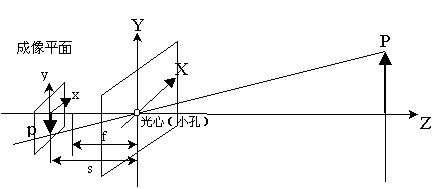
\includegraphics[width=.7\linewidth]{pinhole.jpeg}
  \caption{小孔成像原理示意图}
  \label{fig:pinhole}
\end{figure}

考虑到相机将图片从CMOS中读取出来制成完整图片时,xy方向会有不同程度的拉伸,因此,我们分别
使用两个参数$f_x, f_y$ 表示x方向和y方向上的光心,正常情况下,$f_x f_y$ 即使相互不同也不应当
相差太大。另外,在从相机坐标向图片坐标转换时,需要将像平面上的点统一平移一个量,
这样使得所有像点在图片中的坐标均大于0。因此,假设在相机坐标系内我们有一3维世界坐标点
$M = [X, Y, Z]^T$,在
图片中对应的图像坐标为$m = [u, v]^T, \breve{m} = [u, v, 1]^T$,则二者之间的转换可表示为:

\begin{equation}
  \begin{cases}
    u = f_x * \frac{X}{Z} + c_x \\
    v = f_y * \frac{Y}{Z} + c_y
  \end{cases}
\end{equation}


经过整理可得到较为方便书写的版本:

\begin{equation}
  \begin{aligned}
    \begin{bmatrix}
      u \\
      v \\
      1
    \end{bmatrix}
    &= \frac{1}{Z} K M \\
    &= \frac{1}{Z}
    \begin{bmatrix}
      f_x & 0   & c_x \\
        0 & f_y & c_y \\
        0 & 0   &   1
    \end{bmatrix}
    \begin{bmatrix}
      X \\
      Y \\
      Z
    \end{bmatrix}
  \end{aligned}
\end{equation}

其中K包含了单孔模型中相机的所有信息,因此一般又被成为相机的内参矩阵。

\noindent \textbf{一种通用的相机校准模型——Kannala Brant模型}

如~\ref{subsec:pinhole_cam}所示,理想状态下,图片中记录下来的物体形状
应当与真实世界中的物体满足相似关系,但是由于相机透镜的工艺、相机装配
时的误差,真实相机获取的图片中会发生畸变。Kannala Brant模型
\cite{kannala2006generic} 提供了一种较为普遍且有效的畸变拟合手段,在
工程实践中被广泛的应用在窄视角以及鱼眼相机的正畸过程中。

按照畸变产生的效果来分,主要存在两种畸变,分别是径向畸变及切向畸变。
径向畸变产生的主要原因为相机透镜的折射率无法做到完全一致,径向畸变是
以图像中心为中心,按点到中心的绝对距离r为半径对称分布的,一般来说,径向
畸变有桶型和枕型两种,两种畸变如图~\ref{fig:radial_distort}所示。尽管
两种径向畸变在表现上 不太一样,但是在使用Kannala Brant模型时,可以
使用同一种近似手段来拟合两种畸变。

\begin{figure}[h] % use float package if you want it here
  \centering
  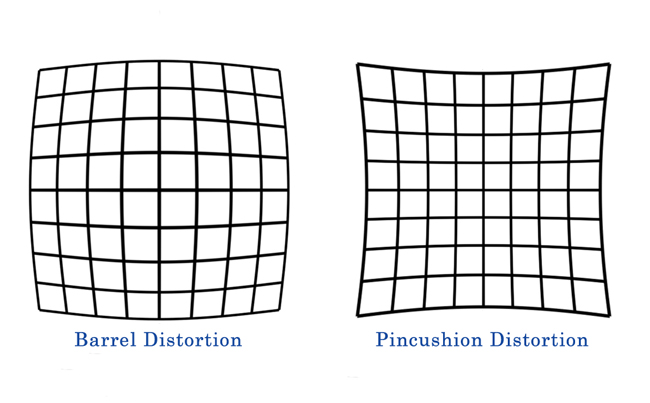
\includegraphics[width=320pt]{camera_distortion.jpg}
  \caption{左桶型畸变,右枕型畸变}
  \label{fig:radial_distort}
\end{figure}

切向畸变则是由于相机装配过程中,相机透镜平面与CMOS感光平面不完全平行造成
的,具体形成原因如图~\ref{fig:tangential_distort}所示。尽管在各种相机校准
方法中,关于切向畸变 都有对应的处理手段,但是在实际工程应用中,由于切向
畸变一般较小,影响也 较小,大多数情况下都不予处理。Tinker的标准
校准流程中,对切向 畸变也不予处理。

\begin{figure}[h] % use float package if you want it here
  \centering
  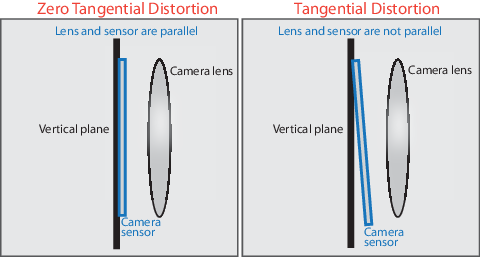
\includegraphics[width=300pt]{tangential_dist.png}
  \caption{左正常装配结果,右有装配误差的装配结果}
  \label{fig:tangential_distort}
\end{figure}

Kannala Brant模型使用光线的入射角$\theta$对图片上对应点的径向距离r进行拟合,
拟合形式如下式所示。

\begin{equation}
  r(\theta) = k_1\theta + k_2\theta^{3} + k_3\theta^{5} + k_4\theta^{7} + ...
\end{equation}

根据工程实践经验,使用KB模型校准时,一般将$k_1$取为1,并对
拟合参数{k}取到5阶,即有效畸变参数为$[k_2, k_3, k_4, k_5]$。

\noindent \textbf{便捷的棋盘格标定——张正友标定法}

张正友标定法~\ref{zhang2000flexible}是种使用方便,应用极其广泛的单摄像头内参标定算法,此标定
法使用前文中提到的Kannala Brant模型,且忽略切向畸变。张正友标定法在使用时仅需执行下列几个
简单的步骤:

\begin{itemize}
  \item 固定摄像头
  \item 打印预先准备好的标定板,确认标定版的尺寸正确、表面平整
  \item 将标定板放置于摄像头视野范围内,变换位置并不断拍摄图片,记录图片信息
  \item 运行标定算法,得到相机内参
\end{itemize}

张正友标定法本质上是利用了标定板上特征点全部位于同一平面的约束:由于一个标定板上的特征点数目
远大于相机内参和约束自由度的总和,因此可以大致估计出相机的内参;在此基础上,再使用最大似然的
思想,最小化所有图片中所有特征点的重投影误差,即可得到精度较高的内参。

我们设标定板上的特征点在世界坐标下的增广坐标为 $\tilde{M} = [X, Y, Z, 1]^T$ ,图片中的增广坐标为$\tilde{m} = [u, v, 1]^T$,世界坐标到相机坐标的位姿变换为$[R, t]$,相机内参矩阵为$K$,尺度因子
为$s$(根据前文单孔成像原理的介绍,这里的s即为相机坐标下点的Z轴坐标),在不考虑
畸变的情况下有:

\begin{equation}
  \begin{aligned}
  	s \tilde{m} &= K 
		\begin{bmatrix}
			R & t
		\end{bmatrix}
		\tilde{M} \\
	s
  	\begin{bmatrix}
  		u \\
  		v \\
  		1
  	\end{bmatrix} &= 
  	\begin{bmatrix}
  		\alpha & \gamma & u_0 \\
  		0      & \beta  & v_0 \\
  		0      & 0      & 1
  	\end{bmatrix}
  	\begin{bmatrix}
		R & t
	\end{bmatrix}
	\begin{bmatrix}
		X \\
		Y \\
		Z \\
		1
	\end{bmatrix}
  \end{aligned}
\end{equation}

由于世界坐标我们可以随意选择,因此我们可以将平面的约束条件直接设为$Z = 0$,那么有:

\begin{equation}
  \label{equ:cam}
  \begin{aligned}
	s
  	\begin{bmatrix}
  		u \\
  		v \\
  		1
  	\end{bmatrix}
  	&= K
  	\begin{bmatrix}
		r_1 & r_2 & r_3 & t
	\end{bmatrix}
	\begin{bmatrix}
		X \\
		Y \\
		0 \\
		1
	\end{bmatrix} \\
	&= K
	\begin{bmatrix}
		r_1 & r_2 & t
	\end{bmatrix}
	\begin{bmatrix}
		X \\
		Y \\
		1
	\end{bmatrix}
  \end{aligned}
\end{equation}

我们设$H = \lambda K [r1, r2, t], H = [h_i, h_2, h_3]$,这里H可以看作标定板真实平面坐标
与图片坐标之间的单应矩阵。将H带入式~\ref{equ:cam},则有:

\begin{equation}
	\label{equ:solve_h}
	s' \tilde{m} = H \tilde{M}
\end{equation}

H是一个3x3的矩阵,有9个元素,但由于H本身是up-to-scale的,因此可以看作有8个自由度。由于我们
知道标定板的真实尺寸,以及标定板中每一个特征点的位置坐标,且世界坐标是我们自己选择的,
我们可以轻易的得到$\tilde{M}$,而$\tilde{m}$是直接从图片中得到的,一般真实的标定板中的特征点数目都远大于8,因此可以通过式~\ref{equ:solve_h}直接求出H各个元素的值。

求解出H后,继续考察式~\ref{equ:cam},根据旋转矩阵的性质,应当有:

\begin{equation}
	\label{equ:const1}
		h_1^T K^{-T} K^{-1} h_2 = 0
\end{equation}

\begin{equation}
	\label{equ:const2}
	h_1^T K^{-T} K^{-1} h_1 = h_2^T K^{-T} K^{-1} h_2
\end{equation}

为了方便下面的计算,我们设$B = K^{-T} K^{-1}$,则B应当是一个对称阵,我们可以根据标定板
上特征点的约束逐个解出B的所有元素,然后反求出K的全部参数。继续推导,我们有:

\begin{equation}
  \begin{aligned}
  	B &=
  	\begin{bmatrix}
  		B_{11} & B_{12} & B_{13} \\
  		B_{12} & B_{22} & B_{23} \\
  		B_{13} & B_{23} & B_{33}
  	\end{bmatrix} \\
  	b &=
  	\begin{bmatrix}
		B_{11} & B_{12} & B_{22} & B_{13} & B_{23} & B_{33}
  	\end{bmatrix}
  \end{aligned}
\end{equation}

\begin{equation}
  \begin{aligned}
  	h_i^T B h_j &= 
  	\begin{bmatrix}
  		h_{i1}h_{j1} & h_{i1}h_{j2} + h_{i2}h_{j1} & h_{i2}h_{j2} &
  		h_{i1}h_{j3} + h_{i3}h_{j1} & h_{i3}h_{j2} + h_{i2}h_{j3} & h_{i3}h_{j3}
  	\end{bmatrix}
  	b \\
  	&= v_{ij}^T b
  \end{aligned}
\end{equation}

则带入约束式~\ref{equ:const1}、~\ref{equ:const2},可以得到:

\begin{equation}
	\label{equ:const_final}
	\begin{bmatrix}
		v_{12}^T \\
		(v_11 - v_22)^T
	\end{bmatrix}
	b = 0
\end{equation}

对于一个有n个特征点的标定板,每一个特征点可以组成一个式~\ref{equ:const_final},则我们可以
轻易的解出b中的每一个元素的值。b解出后,K中的每一个参数都可以通过b的元素唯一的反算出来,其具体
形势可见~\cite{zhang2000flexible}这里不再描述。

下面我们考虑畸变参数。通常我们假设畸变是比较小的(当然,这一假设很多时候都不怎么对),那么对于
一个在相机坐标系下真实位置为$[\breve{x}, \breve{y}, \breve{z}]$的点,其畸变后的坐标为
$[x, y, z]$,则在对径向畸变做二阶近似的情况下,我们有:

\begin{equation}
  \begin{aligned}
  	\breve{x} &= x + x[k_1(x^2 + y^2) + k_2(x^2 + y^2)^2] \\
  	\breve{y} &= y + y[k_1(x^2 + y^2) + k_2(x^2 + y^2)^2]
  \end{aligned}
\end{equation}

那么投影到图片坐标中,应当有

\begin{equation}
  \begin{aligned}
  	\breve{u} &= u + u[k_1(x^2 + y^2) + k_2(x^2 + y^2)^2] \\
  	\breve{v} &= v + v[k_1(x^2 + y^2) + k_2(x^2 + y^2)^2]
  \end{aligned}
\end{equation}

由前文的推导我们可以知道,当我们解出了单应矩阵H、且知道标定板的真实尺寸时,其实每一个特征点
在相机坐标下的位置就已经得到了,整理前式,可得


\begin{equation}
	\label{equ:dist}
	\begin{bmatrix}
		(u - u_0)(x^2 + y^2) & (u - u_0)(x^2 + y^2)^2 \\
		(v - v_0)(x^2 + y^2) & (v - v_0)(x^2 + y^2)^2
	\end{bmatrix}
	\begin{bmatrix}
		k_1 \\
		k_2
	\end{bmatrix}
	=
	\begin{bmatrix}
		\breve{u} - u \\
		\breve{v} - v
	\end{bmatrix}
\end{equation}

实际计算中,可将各个特征点的信息带入求得最小二乘意义下的$[k_1, k_2]$的解,之后将这个解
同前文所述的H以及K的各个参数作为优化处置,共同求解一个最小化重投影问题:

\begin{equation}
	\sum_{i=1}^{n}\sum_{j=1}^{m} \| m_{ij} - \breve{m}(K, k_1, k_2, R_i, t_i, M_j)\|^2
\end{equation}

上式的意义为,对于有n张图片,每张图片m个特征点的标定问题,对于每一张图片的每一个特征点$m_{ij}$,
计算其真实坐标点到图片平面的投影$\breve{m}(K, k_1, k_2, R_i, t_i, M_j)$,并对两者的误差进行
优化,实践中我们一般使用Levenberg-Marquardt方法来求解。

张正友标定法给出了非常方便的单一摄像头内参标定方法,但是在实践中,有时我们不但需要准确的摄像头内参校准,
还需要对不同传感器进行时间对齐,这项技术目前已经有非常成熟的发展,如文\cite{furgale2013unified, furgale2012continuous}所述,基于这项技术的开源标定库Kalibr\cite{rehder2016extending}在学术界
和工业界都有广泛的应用。对于多模态移动机器人来说,有时候也需要基于时间对齐的标定技术,但由于其本身内容
较多,这里不再另外介绍。

\subsection{摄像头外参标定(手眼标定)}

摄像头是机器人的眼睛,而机器人作为多传感器、多执行部件组成的整体,摄像头主要部件(比如光心)
相对机器人的安装位置的精确标定是十分重要的,好的外参标定是机器人出色表现的基石。根据业界通用
规范,按安装位置的不同机器人的摄像头外参标定可以分两种:eye-on-hand,eye-on-base。这两
种摄像头安装方式虽然不同,但可以统一到一个标定框架下,使用一套标定求解算法进行求解,只是在
某些参数的设置上需要互换位置。

\noindent \textbf{eye-on-base安装法}

这种摄像头安装位置指代的是将摄像头安装在某个同机械臂的底盘刚性连接的位置上,Tinker的头部
Kinect就是一个典型的的eye-on-base安装的摄像头。典型的eye-on-base安装方式如图\ref{fig:eye_on_base}
所示。

\noindent \textbf{eye-on-hand安装法}

这种安装方式一般是指将摄像头安装在机械臂的末端,一般在夹爪的腕部。这样可以提高末端的执行精度,
改善机器人的表现。典型的eye-on-hand安装方式如图\ref{fig:eye_on_hand}所示。

\begin{figure}
\centering
\begin{subfigure}{.5\textwidth}
  \centering
  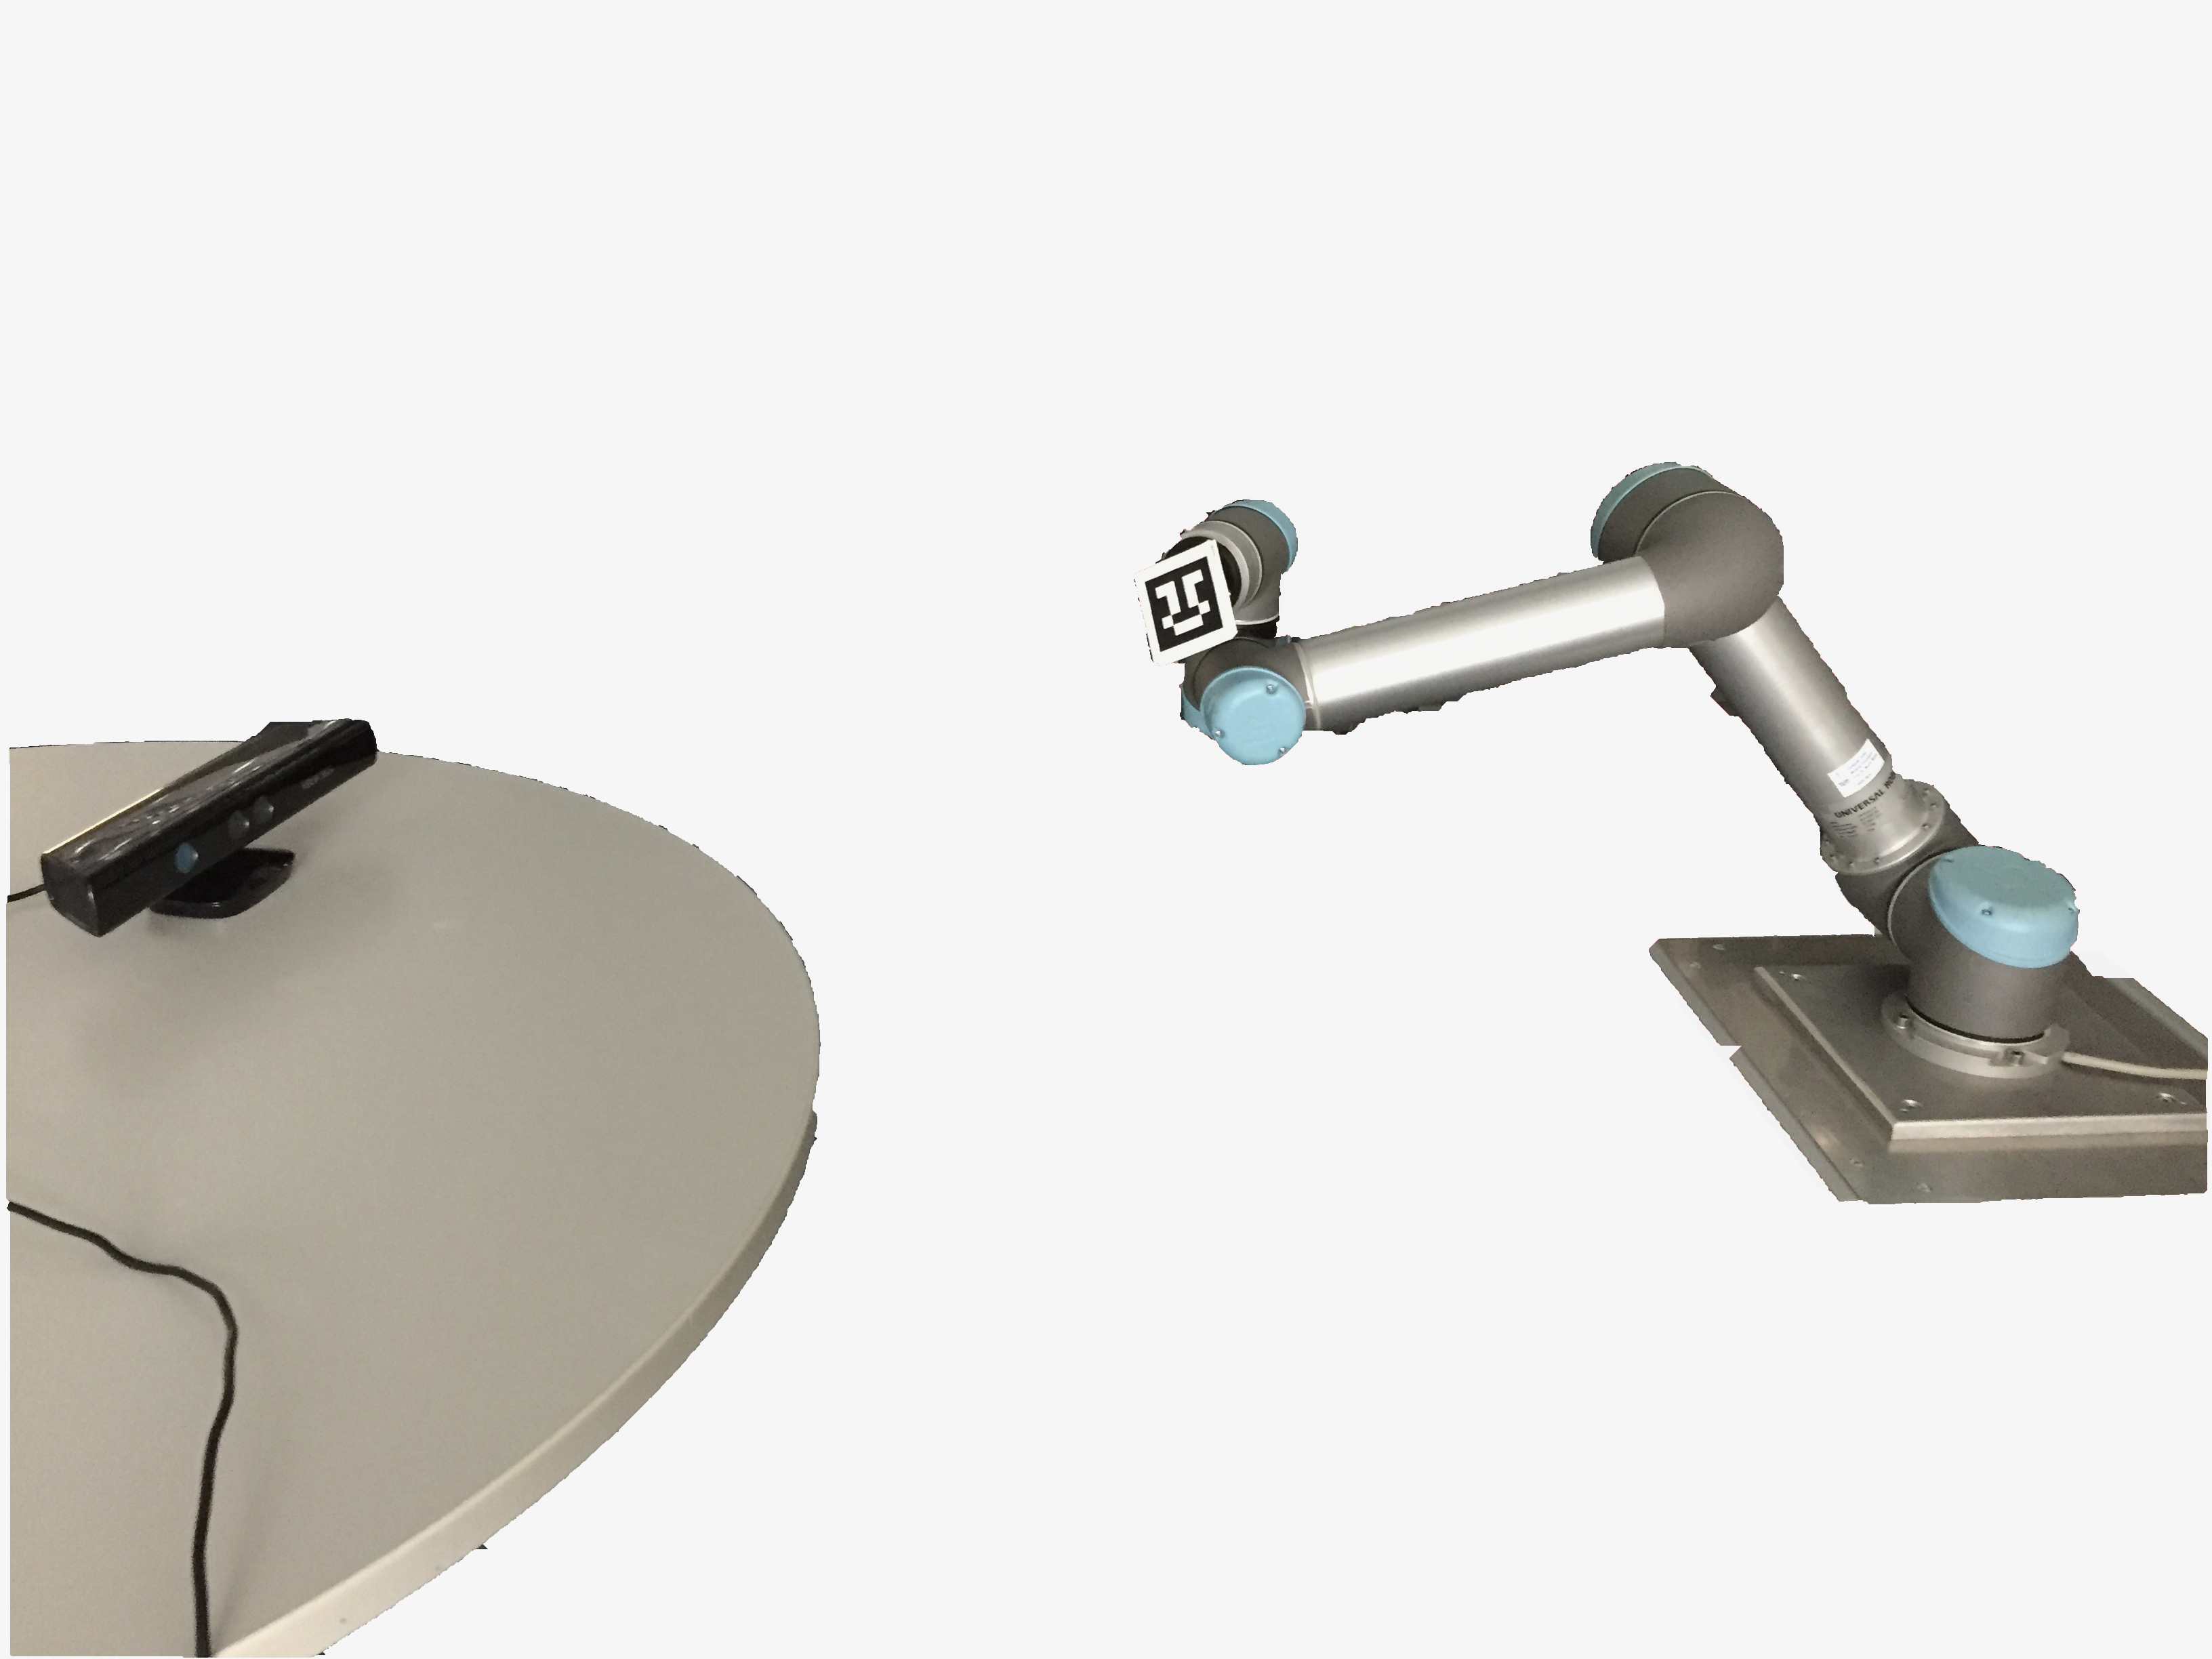
\includegraphics[height=4cm]{eye_on_base_aruco_pic.png}
  \caption{eye-on-base安装示意图}
  \label{fig:eye_on_base}
\end{subfigure}%
\begin{subfigure}{.5\textwidth}
  \centering
  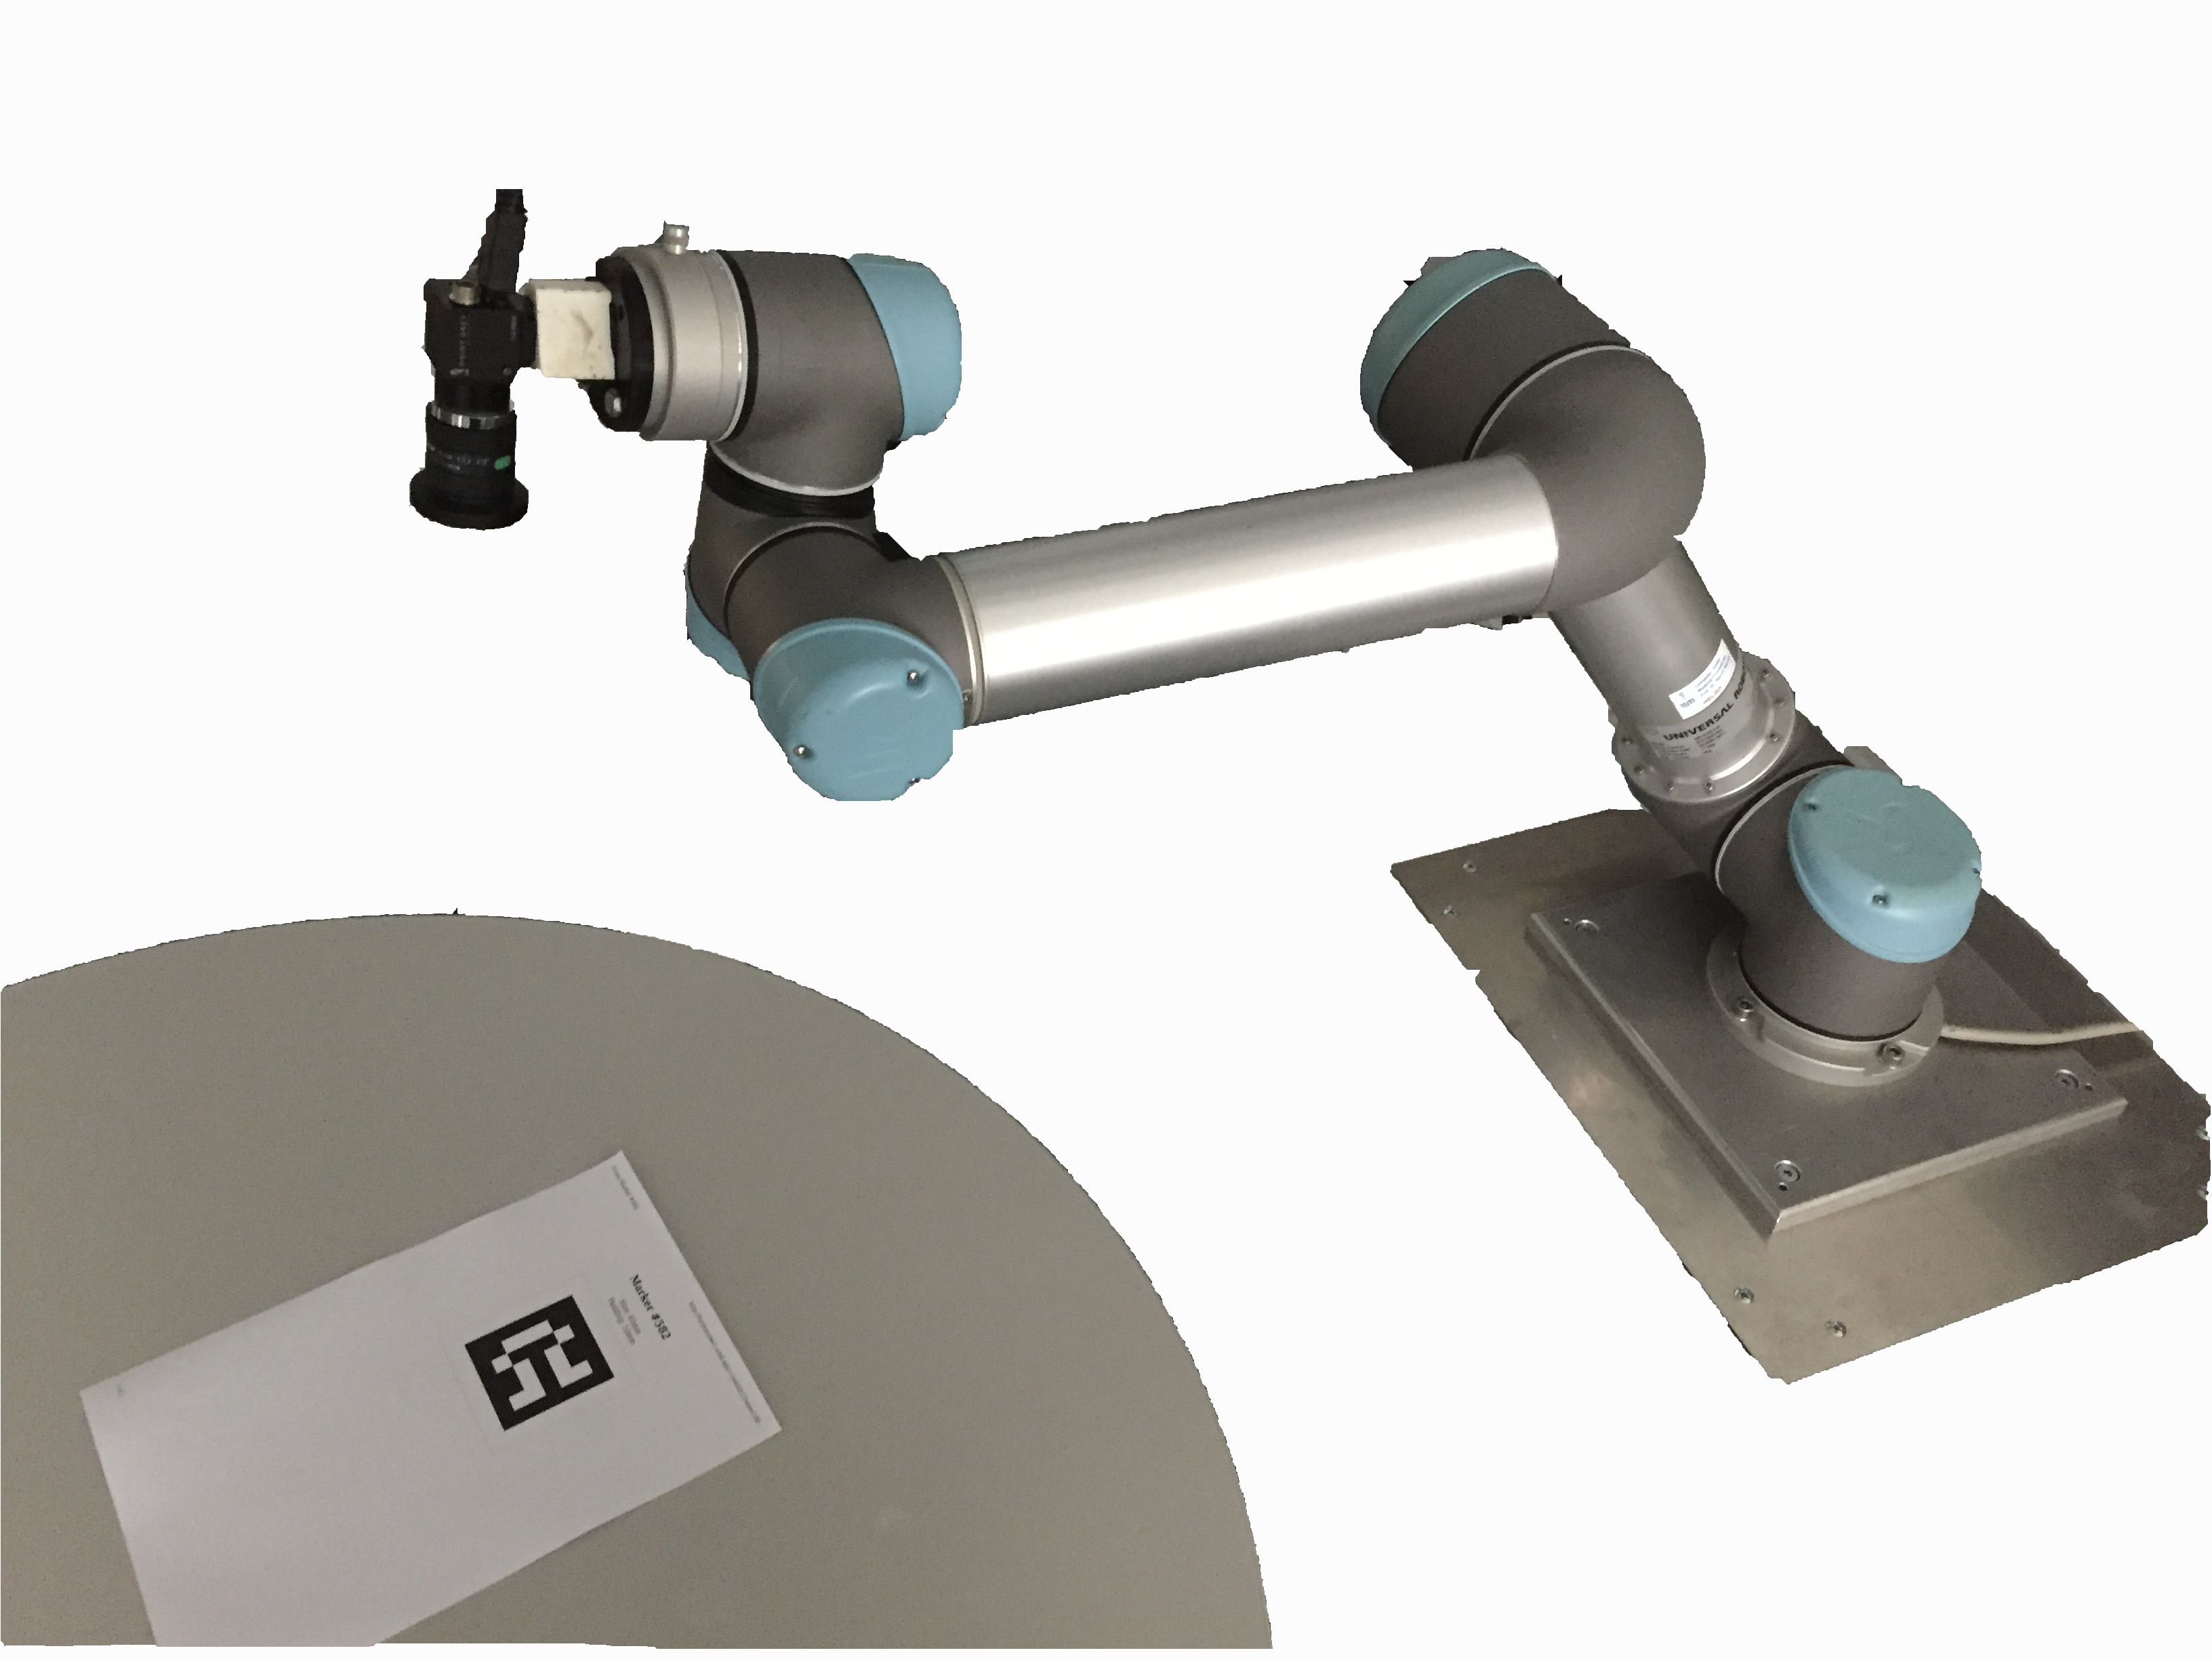
\includegraphics[height=4cm]{eye_on_hand_aruco_pic.png}
  \caption{eye-on-hand安装示意图}
  \label{fig:eye_on_hand}
\end{subfigure}
\caption{手眼标定的典型安装方式,图片来源\cite{easy_handeye}}
\end{figure}


\noindent \textbf{标定方法介绍}

对于这两种安装方法来说,我们希望知道的是相机光心相对机器人某个特定位置的准确坐标变换,直接
测量显然是不现实的,但是由于机械臂是一种可以提供精确的位置变换的部件,我们可以利用这一部件和
摄像头本身的检测能力解算出准确的位置变换。

标定时,我们需要一个外部锚点作为参照,通常会使用Aruco码\cite{garrido2014automatic}
作为锚点。Aruco码是一种预先设计好尺寸
和纹理的二维图案,程序通过边缘检测和匹配,可以在预先知道码号和码的物理尺寸的情况下,准确的通过
二维相机中的图像恢复出码中心相对相机光心的位姿。如图\ref{fig:aruco}所示,Aruco检测程序不单
能准确的解算出码的三维位置,也可以求解出码的姿态。

\begin{figure}[h] % use float package if you want it here
  \centering
  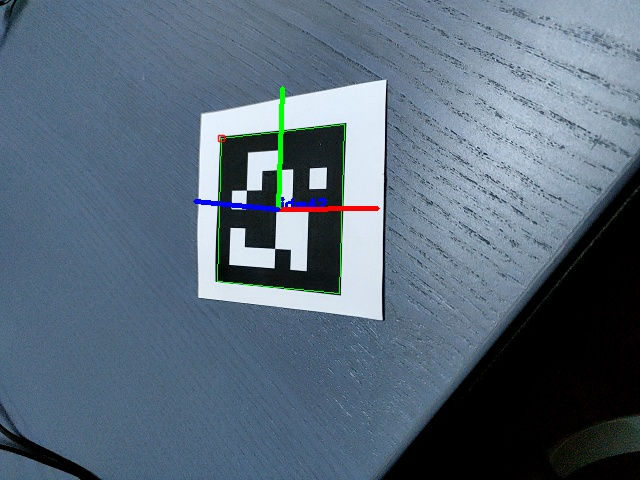
\includegraphics[width=300pt]{aruco.jpg}
  \caption{Aruco码的三维定位效果,图片来源\cite{aruco}}
  \label{fig:aruco}
\end{figure}

我们先来分析eye-on-base的情况,如图~\ref{fig:hand_eye}所示,对于一个相机相对机
械臂底盘安装的模型来说,应当有:

\begin{equation}
  T_{cam\_aruco} * T_{aruco\_hand} * T_{hand\_base} = T_{cam\_base}
\end{equation}

\begin{figure}[h] % use float package if you want it here
  \centering
  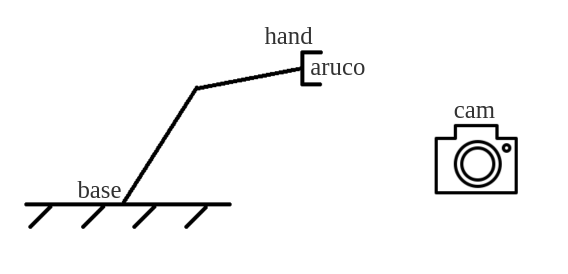
\includegraphics[width=300pt]{hand-eye.png}
  \caption{手眼标定模型示意图}
  \label{fig:hand_eye}
\end{figure}

其中$T_{cam\_aruco}$代表从相机光心到Aruco码中心的坐标变换,$T_{aruco\_hand}$代表
Aruco码中心到机械臂末端的变换,因为Aruco码并不是精确放置的这部分我们通常既不知道,也不关心,
而且在整个标定过程中,这个量也不会变化,$T_{hand\_base}$是指机械臂底盘到末端的变换,这部分
应当由机械臂本身给出,$T_{cam\_base}$是相机到底盘的变换,我们的目标变换是它的逆$T_{base\_cam}$,经过适当变换后,我们可以得到:

\begin{equation}
  \begin{aligned}
    T_{aruco\_hand} &= T_{cam\_aruco}^{-1} * T_{cam\_base} * T_{base\_hand} \\
    T_{hand\_aruco} &= T_{base\_hand}^{-1} * T_{base\_cam} * T_{cam\_aruco}
  \end{aligned}
\end{equation}

当我们有两个测量,且这两个测量中机械臂的位姿不同时,可以通过联立将式的
未知量$T_{hand\_aruco}$消去,并得到:

\begin{equation}
  T_{base\_hand}^{(1)-1} * T_{base\_cam} * T_{cam\_aruco}^{(1)} = 
  T_{base\_hand}^{(2)-1} * T_{base\_cam} * T_{cam\_aruco}^{(2)}
\end{equation}

经过整理可得:

\begin{equation}
  T_{base\_hand}^{(2)} * T_{base\_hand}^{(1) -1} * T_{base\_cam}= 
  T_{base\_cam} * T_{cam\_aruco}^{(2)}  * T_{cam\_aruco}^{(1) -1} 
\label{equ:eye_on_base}
\end{equation}

由于$T_{case\_hand}$和$T_{cam\_aruco}$都是由测量获得,每次的结果也不一样,则
$T_{case\_cam}$的求解问题就被简化成了经典的三维欧氏流型上的$AX = XB$求解问题了,
这种问题有固定的处理方式,如\cite{park1994robo}所述,还有完备的数学手段通过
使用统计手段增加测量组数以提高精度\cite{tsai1989new}。

对于eye-on-hand的情况,我们同样可以仿照上文建立坐标变换方程,经过整理可以得到
约束关系为:

\begin{equation}
  T_{base\_hand}^{(2) -1} * T_{base\_hand}^{(1)} * T_{hand\_cam}= 
  T_{hand\_cam} * T_{cam\_aruco}^{(2)}  * T_{cam\_aruco}^{(1) -1} 
\label{equ:eye_on_hand}
\end{equation}

可以看到,上式与~\ref{equ:eye_on_base}的形式非常相似,只是$T_{base\_hand}$
为前式的逆,因此在实际操作中,两种标定类型通常共用一套求解程序,只是在获取base到
hand的参数时将顺序置换一下。

为方便机器人的组装与调整,Tinker团队为其摄像头的手眼标定流程开发了自动化控制程序。
标定头部相机时,机器人将aruco码直接夹在夹爪末端,以一定概率拉取仓库中硬编码好的
标定位姿或者随机生成位姿,不断重复记录数据并且解算,得到头部相机的外参;标定机器人
腕部相机时,机器人直接将码放置在桌面上,如前文所示不断变换位姿记录数据,完成标定
流程。每次机器人各部件位置调整后,只需一键运行标定程序,机器人即可自动完成标定程序,
省时省力,如图~\ref{fig:tinker_calib} 机器人在执行自动标定任务。

\begin{figure}[h] % use float package if you want it here
  \centering
  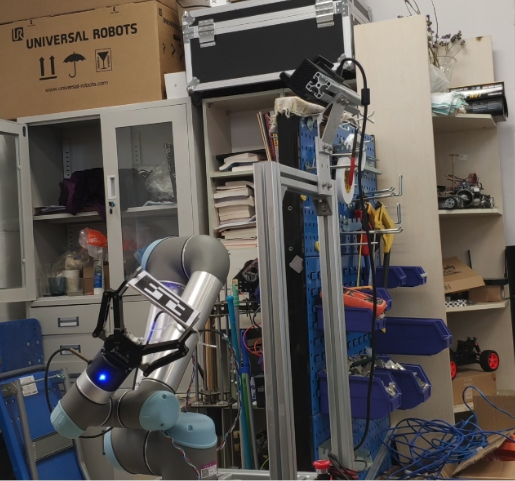
\includegraphics[width=340pt]{tinker_calib.png}
  \caption{Tinker在执行自动标定程序}
  \label{fig:tinker_calib}
\end{figure}


\section{视觉定位与识别}

对于多模态灵巧操作机器人来说,视觉功能非常重要。在实际控制中,我们通常将物品的定位与识别
划分为两个不同的部分,他们对应的后续处理也不同:视觉识别主要解决这个东西是什么、可不可以抓、
抓了之后怎么办的问题;而视觉定位则需要告诉后面的程序当前目标在三维空间的什么位置,它是什么形状,以
什么姿态存在。

一般情况下,多模态机器人获取物品位置信息的主要手段是RGBD相机,通过头部或者手部的RGBD摄像头,
机器人可以通过某些算法拿到物品相对相机光心的精确位置,再依赖准确的手眼标定通过坐标变换得到
物品理想的坐标信息。

大部分情况下,目标物品是离散的放置在桌子或者柜子中的,上游程序将机器人导航到合适的位置后,可以
将机器人的头部摄像头大致的对准目标,然后交由定位程序接管。定位程序从头部RGBD摄像头中拿到点云
信息后,会依据先验知识对场景进行分割。例如若目标物品放在一张桌子上,那么这张桌子大致的高度,
形状,大小对于程序来说都应当是已知的,那么程序就可以通过平面分割辅以平面参数检验的方式在场景
中高概率的找出桌子所在的平面;当目标放在柜子上时原理与前文相似,但是要注意柜子的平面相比而言
要更加复杂一些。将桌子或者柜子平面所包含的点云去除后,我们可以接着利用桌子的相关参数,将
桌面以上我们感兴趣的一小块区域裁剪出来。此时我们得到的点云就已经比较良好了,之后可以直接对物品
进行聚类,或者使用视觉识别程序的结果将不同物品对应的框筛查出来再进行聚类,甚至利用类似Mask-RCNN
等可以生成Mask Segment的技术直接将对应的点云抠出来,再做质心检测和三维重建。

TODO:segmentation分步骤的演示图

关于物品的识别技术,机器人领域完全仰仗近些年来深度学习机器视觉的发展。对于摆放在
桌面上离散分布的物品,我们一般使用Yolo、Fast-RCNN或者Mask-RCNN等等深度学习的检测算法
进行分类。这些算法本身有开源实现且有经过大规模训练的初始参数,当机器人要面对特殊物品时,通常
会针对这一类物品重制数据集,在原有模型的基础上进行Fine Tune,一般就可以获得非常好的效果。

TODO:Fine tune过后物品的框图效果

\section{抓取点选择}

抓取点的选取并不是一个普遍存在的需求,例如在机器人不执行抓取任务,而是单纯完成某些动作的时候。
或者机器人抓取的物品形状规则、位置离散时。但是,对于密集堆放的物品的pick-up任务,抓取点的选择
对于机器人性能至关重要。

在实际操作中对抓取点要求不高时,可以采用一种简单的实现方式,即定位出物品质心后,将抓取位姿简单的
设置为沿机器人与物品质心的连线且平行于桌面。但是复杂的抓取任务需要一些较为复杂的抓取点选择算法。
下面介绍比较常用的二指夹爪抓取点算法GPD(Grasp Pose Detection)\cite{ten2017grasp}的实现方式。

TODO:沿线抓取的效果图视频

GPD算法的大致流程是:使用随机生成方式生成大量抓取位姿;之后使用训练过的CNN选择器筛选出其中较优
的抓取位姿。算法中,CNN选择器的设置是比较考究的,对于每一个抓取位姿如图~\ref{fig:gpd}所示,
算法都会在x,y,z方向分别
投影,抽取出夹爪在这三个方向上平移时可以直接触碰到的物品的表面的点云投影到三个方向,制作成图片
输入CNN网络中。

\begin{figure}[h] % use float package if you want it here
  \centering
  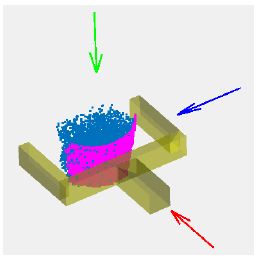
\includegraphics[width=300pt]{gpd.png}
  \caption{GPD将位姿输入CNN时的处理方式示意}
  \label{fig:gpd}
\end{figure}

作为一个判别网络,这个CNN结构在训练时使用的判别技术也很有趣:它的训练标准是通过评价一个抓取位姿的
摩擦吻合程度和对心程度实现的。如图~\ref{fig:fa_grasp}展示了一个标准的无摩擦对心夹取位姿,即物品
与夹爪的两个接触点的法向最好与夹爪平面垂直,并且两个接触点法向的连线最好共线。通过直观的思考,我们
可以感觉到,这种筛选方式是合理的,无摩擦对心夹取在人类动作中也非常常见,而且是夹起外形复杂的物品的
有力保证。


\begin{figure}[h] % use float package if you want it here
  \centering
  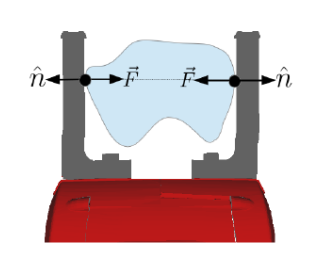
\includegraphics[width=300pt]{fa_grasp.png}
  \caption{无摩擦对心夹取(fractionless antipodal grasp)}
  \label{fig:fa_grasp}
\end{figure}

除了上文的GPD之外,一些基于吸盘的抓取点选择算法也广受关注,吸盘或者吸盘夹爪配合法在物流分捡中有比
移动机器人方向更加广泛的应用。近年来,一些基于CNN生成吸取点的算法广受关注,如在Amazon Picking 
Challenge中由MIT-Printceton队开发的兼顾抓取点与吸取点生成的算法\cite{zeng2018robotic}就
取得了令人瞩目的成绩(如图~\ref{fig:mit_princeton},MIT-Princeton的算法在赛场上)

\begin{figure}[h] % use float package if you want it here
  \centering
  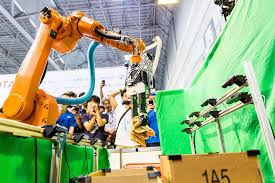
\includegraphics[width=340pt]{mit_princeton.jpeg}
  \caption{MIT-Princeton机器人夹起一条毛巾}
  \label{fig:mit_princeton}
\end{figure}

\section{机械臂运动规划}

机械臂的运动规划是多模态机器人控制中最为关键的一环。当我们通过视觉方法得到了目标物品
的三维位姿并解算出最优抓取点后,我们通常得到的是夹爪末端某个位置的位姿,那么如何准确的控制
机械臂运动到目标位置,并且不碰撞到机器人自己或者环境中已知的任何障碍呢?

通常从目标位姿到实际控制的过程在编码层面被划分为三步:逆运动学阶段(IK,Inverse Kinematics),
路径寻找与后处理,运动控制。

\noindent \textbf{逆运动学求解}

逆运动学阶段的作用是将我们给出的末端位姿转换成合法的机械臂各个关节的角度,如图\ref{fig:ik}展示
了一个简易的二自由度机械臂逆运动学求解的结果。对于很多自由度较高
的机械臂来说,一个末端位姿很可能对应若干个合法的解,这些解经过简单的筛选之后,都会被传入到下一个
阶段供求解器使用。IK技术在机器人领域以及计算机动画制作领域都有广泛的应用,对于某些特定的模型(
例如前文提到的二自由度机械臂)其逆运动学结果是有解析解的。但是对于大部分实际机械臂的逆运动学问题
我们还是需要依赖数值方法求解。实际操作中大部分使用类梯度下降的技术对机器人的各个关节进行优化,
不断迭代寻找到误差允许范围内和目标位姿足够接近的解即可。总体来说,IK技术目前已经是一个比较成熟
可靠的方法,机器人领域也有一些可靠的开源方案可供使用,例如2008年发布的OpenRAVE库\cite{diankov2008openrave}
就提供了鲁帮且全面的IK功能,经常被封装成插件应用到各大机械臂规划平台上。

\begin{figure}[h] % use float package if you want it here
  \centering
  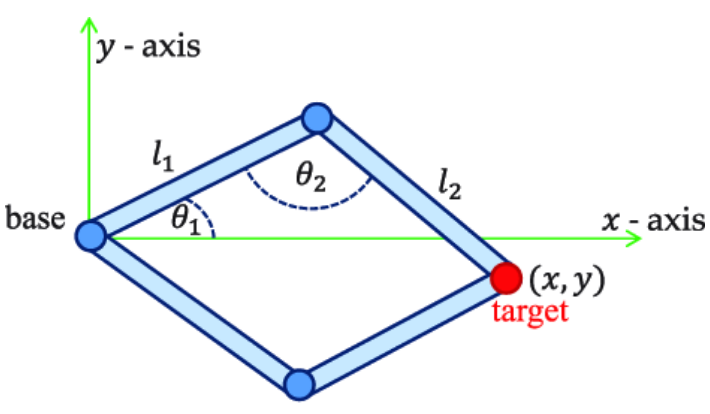
\includegraphics[width=280pt]{ik.png}
  \caption{一个简单的IK求解例子}
  \label{fig:ik}
\end{figure}

\noindent \textbf{轨迹搜索与优化}

路径寻找阶段是指:已知当前机械臂各关节位置以及目标位置,我们应如何找到一个连续的路径,使得机械臂沿着
这一轨迹移动时可以流畅、顺滑且不碰撞到任何已知障碍的到达目标位姿。这一领域目前还在不断的发展,有很多
巧妙的求解方式被不断开发出来\cite{masehian2007classic},但现实开发中,比较常用的还是使用基于采样的
RRT\cite{lavalle1998rapidly}算法。使用RRT算法前需要对整个求解空间进行一定的前处理,具体步骤为:
使用采样的方式在整个解空间内生成出无数可能的位姿每个位姿可视为一个节点,然后通过位姿的邻近关系将这些
节点连通起来,组成一个图结构,并且使用碰撞检测去除那些非法的位姿。完成这些预处理步骤后,就可以利用RRT
算法对解进行搜索。RRT算法全名Rapidly-exploring Random Tree,其核心思想非常简单:从现有位置开始,
在图上维护一颗树,通过某种策略不断的扩展树上的节点直到达到目标位置,或者寻找失败,如图\ref{fig:rrt}
描述了树生长过程中的形态。

\begin{figure}[h] % use float package if you want it here
  \centering
  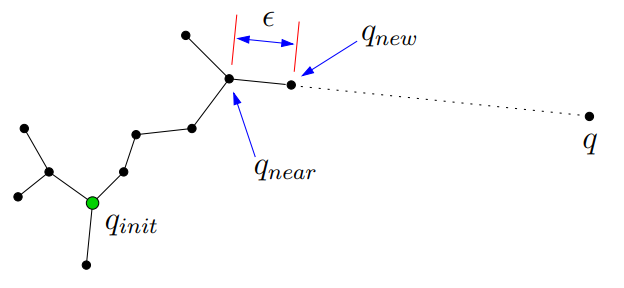
\includegraphics[width=320pt]{rrt.png}
  \caption{RRT算法中树生长的过程\cite{kuffner2000rrt}}
  \label{fig:rrt}
\end{figure}

在RRT树完成搜索后,可以通过回溯的方式找到在解空间内从出发点到目的地的一条连续的轨迹,由于RRT的
工作方式所限,这条轨迹一般比较曲折,需要使用平滑器对轨迹进行平滑并且加入更多插样点。

\noindent \textbf{运动控制}

机械臂的运动控制主要是指:在给出了合理的各关节连续的角度位置后,应当如何控制真实的机械臂设备,使得
它能够及时、准确的到达每一个约定的位置,或者至少是末端位置。这一领域涉及较为复杂的电流、位置控制,
同机械臂的物理尺寸、电路设计电机选择均强相关,一般由机械臂厂商提供,或者直接集成到成品机械臂中。由于
本文主要描述算法相关的机械臂控制问题,因此尽管运动控制问题本身难度大、应用广、研究深入,本文对这一
问题还是不再探讨。


本文给出的多模态机器人基于ROS平台进行开发,ROS下有一个生态比较完全的的机械臂控制框架MoveIt!\citep{chitta2012moveit}
,提供了IK、路径搜索平滑功能,以及完善的可视化调试接口,如图\ref{fig:moveit_viz}。

\begin{figure}[h] % use float package if you want it here
  \centering
  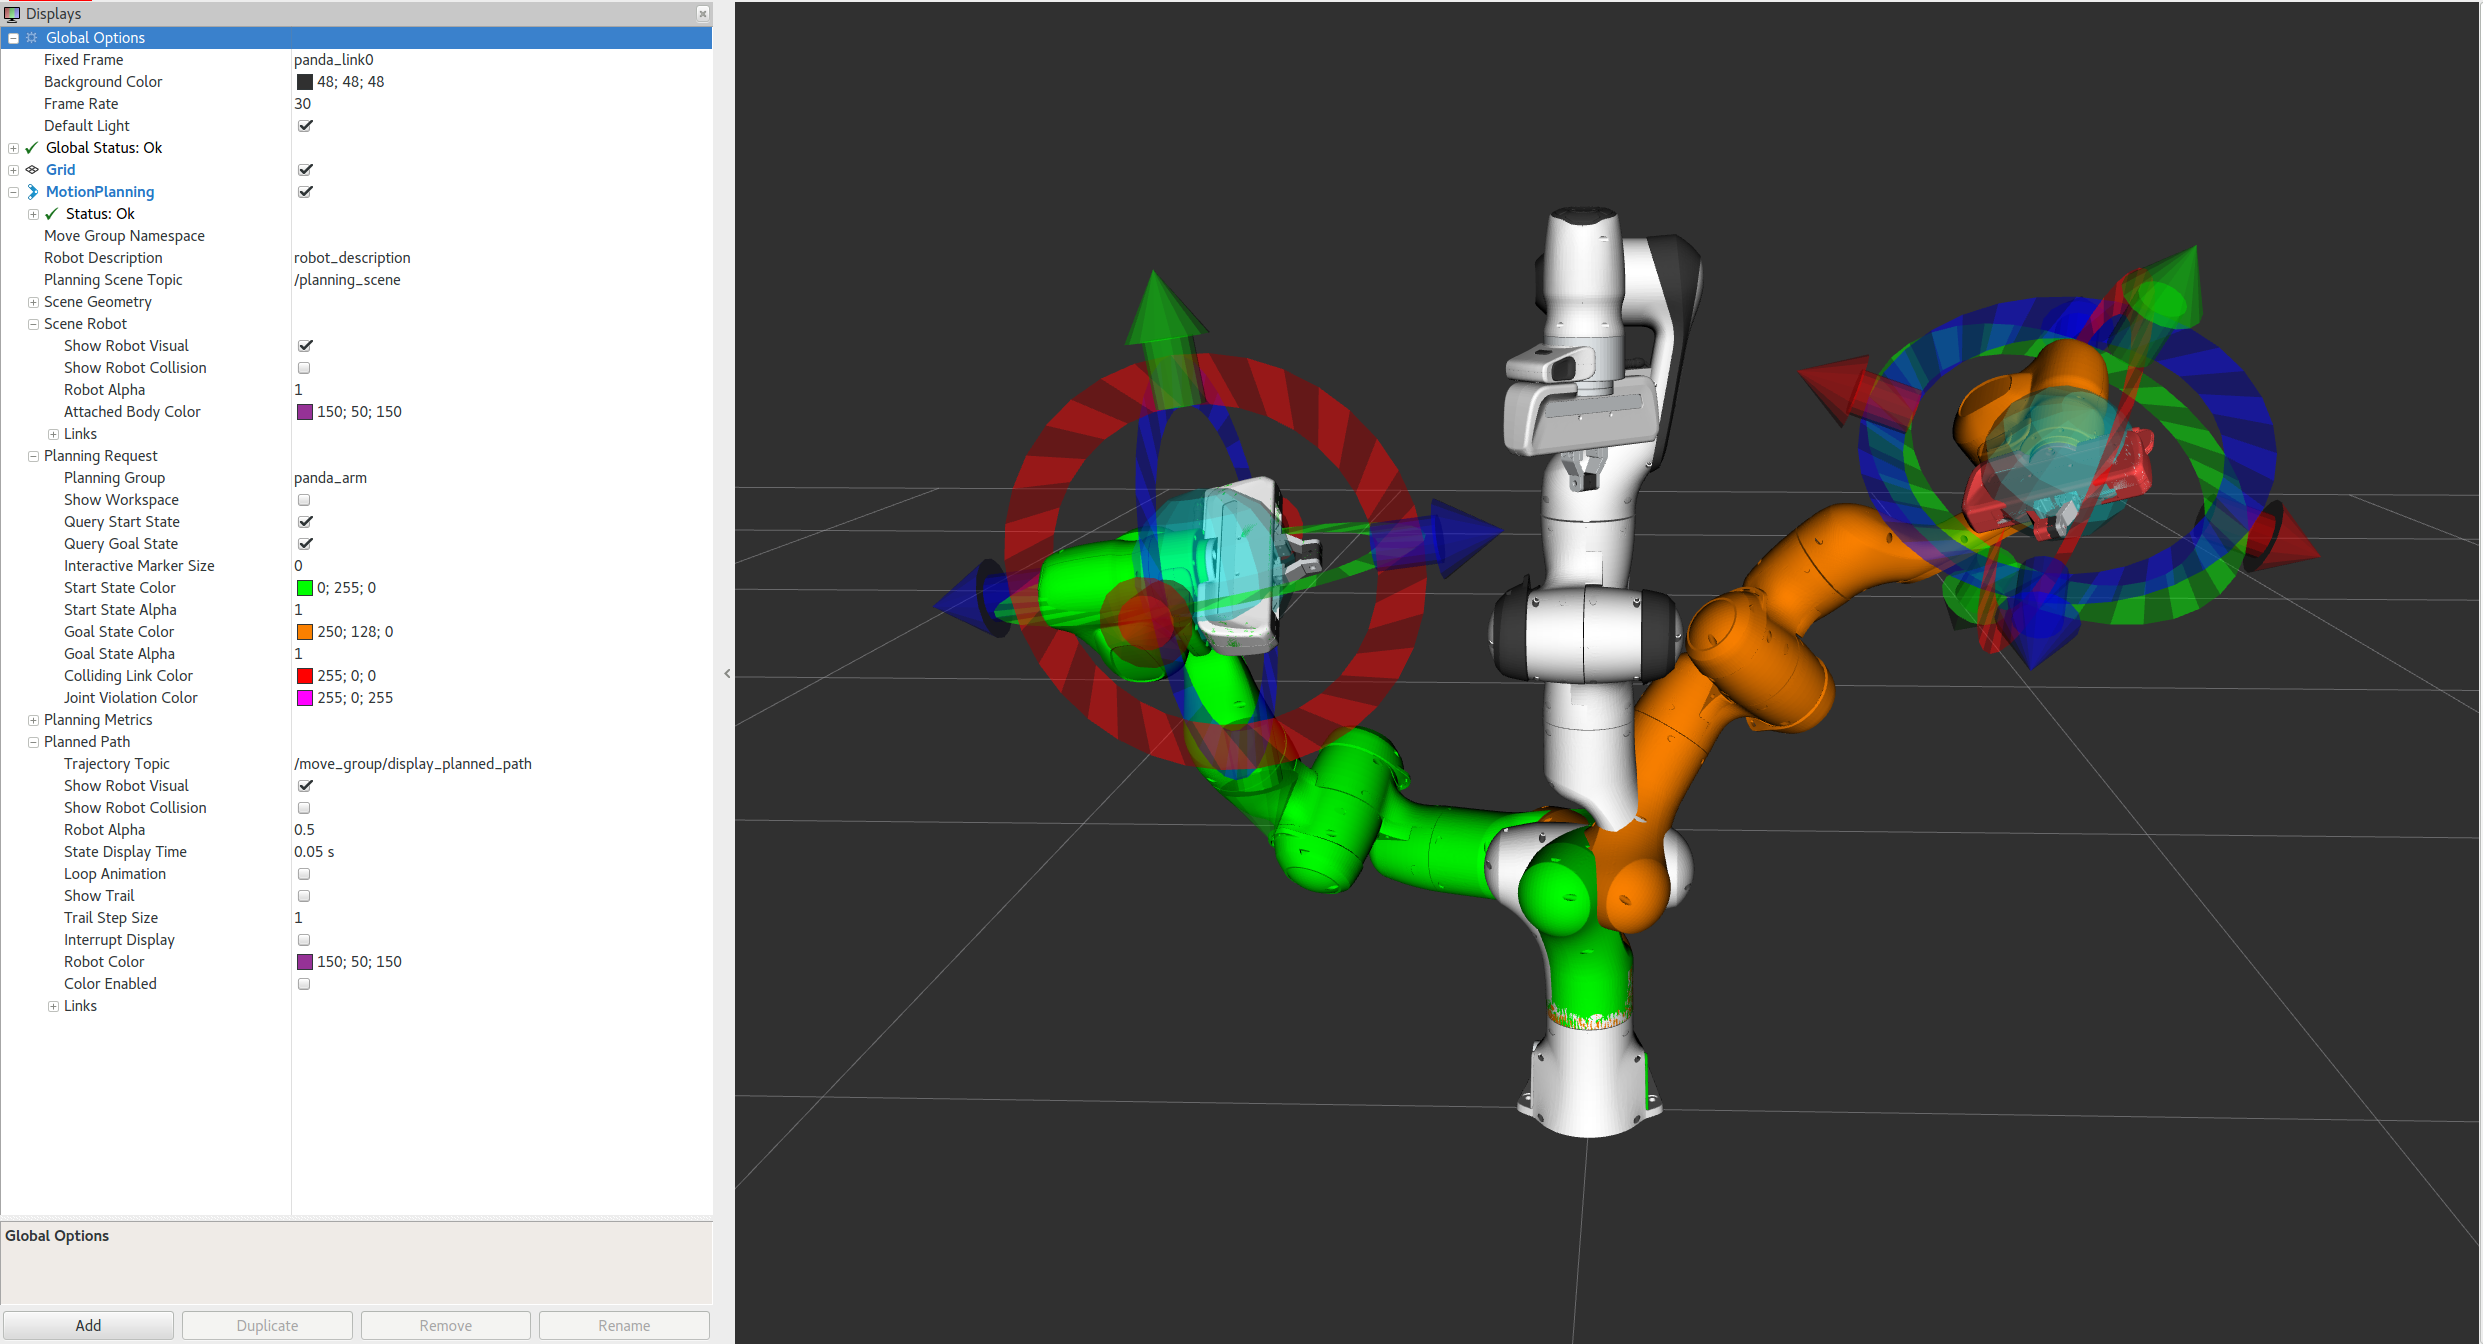
\includegraphics[width=300pt]{moveit_viz.png}
  \caption{MoveIt!的可视化效果}
  \label{fig:moveit_viz}
\end{figure}


\section{本章小结}

本章完整的给出了从摄像头标定到目标物体检测、定位、识别所需要的各项技术,并详细的介绍了机械臂控制
的主要流程与关键技术。每一个关键的技术节点都详细的给出了Tinker机器人使用的具体方案,给出了
复杂场景下移动操作机器人机械臂功能控制的完整技术描述。






















